 % --------------------------------------------------------------
% This is all preamble stuff that you don't have to worry about.
% Head down to where it says "Start here"
% --------------------------------------------------------------

\documentclass[11pt]{article}

\usepackage[margin=1in]{geometry} 
\usepackage{amsmath,amsthm,amssymb}
\usepackage{afterpage}
\usepackage{indentfirst}
\usepackage{graphicx}
\graphicspath{ {images/} }
\usepackage{amsmath}
\usepackage{upgreek}
\usepackage{rotating}
\usepackage{fixltx2e}
\usepackage{float}
\usepackage{gensymb}
\usepackage[section]{placeins}


\numberwithin{equation}{subsection}
%\numberwithin{figure}{section}

\newcommand{\N}{\mathbb{N}}
\newcommand{\Z}{\mathbb{Z}}

\newenvironment{theorem}[2][Theorem]{\begin{trivlist}
		\item[\hskip \labelsep {\bfseries #1}\hskip \labelsep {\bfseries #2.}]}{\end{trivlist}}
\newenvironment{lemma}[2][Lemma]{\begin{trivlist}
		\item[\hskip \labelsep {\bfseries #1}\hskip \labelsep {\bfseries #2.}]}{\end{trivlist}}
\newenvironment{exercise}[2][Exercise]{\begin{trivlist}
		\item[\hskip \labelsep {\bfseries #1}\hskip \labelsep {\bfseries #2.}]}{\end{trivlist}}
\newenvironment{problem}[2][Problem]{\begin{trivlist}
		\item[\hskip \labelsep {\bfseries #1}\hskip \labelsep {\bfseries #2.}]}{\end{trivlist}}
\newenvironment{question}[2][Question]{\begin{trivlist}
		\item[\hskip \labelsep {\bfseries #1}\hskip \labelsep {\bfseries #2.}]}{\end{trivlist}}
\newenvironment{corollary}[2][Corollary]{\begin{trivlist}
		\item[\hskip \labelsep {\bfseries #1}\hskip \labelsep {\bfseries #2.}]}{\end{trivlist}}

\newenvironment{solution}{\begin{proof}[Solution]}{\end{proof}}

\begin{document}
	
	% --------------------------------------------------------------
	%                         Start here
	% --------------------------------------------------------------
	
	\title{Simulink Implementation of a GPS Receiver}
	\author{Alamjyot Parihar 260570908 \\ Ahmed Sami 260568821\\
		Project Supervisor:Prof. Haryy Leib}
	
	\maketitle
	\newpage
	\tableofcontents
	\newpage
	\listoffigures
	\listoftables
	\newpage
	
	\section{Abstract}
	
	Traditionally the algorithms that make up a complete software defined GPS are done in assembly, C/C++ or Matlab. This requires a large team to write and test algorithms, which is both costly and time consuming. This project is intended to provide a basis for clear, easy to follow and modify implementation of a L1 carrier GPS receiver. Our simulation employs the use of the graphical programming environment Simulink to design and test models.This project aims to make the fundamental functionality of a GPS receiver more visible and the inner workings simpler to examine and analyze. We hope that our implementation will help pave the way for other simpler methods of implementing and understanding intricate systems.
	
	\section{List of Abbreviations}
	
	\begin{description}
		\item[CDMA] - Code Division Multiple Access
		\item[BPSK] - Binary Phase Shift Keying
		\item[LO] - Local Oscillator
		\item[C/A] - Coarse/Acquisition
		\item[DLL] - Delay Locked Loop
		\item[PLL] - Phase Locked Loop
		\item [SNR]{Signal to Noise Ratio}]
	\end{description}
	\section{Introduction}
	\section{Overview of Previous Work}
	\subsection{Signal Generator}
	
	\subsection{Acquisition Loop}
	
	
	\section{Doppler Shift}
	
	Due to the nature of satellite navigation systems, the point of signal generation is constantly moving overhead. This movement causes a doppler effect on the signal, leading to shifts in carrier frequency and code phase seen at the receiver. Typically, doppler shifts to code phase can reach up to $\pm3$ chips/s for stationary receivers.
	\section{Signal Generation}
	
	\begin{figure}
		\centering
		
		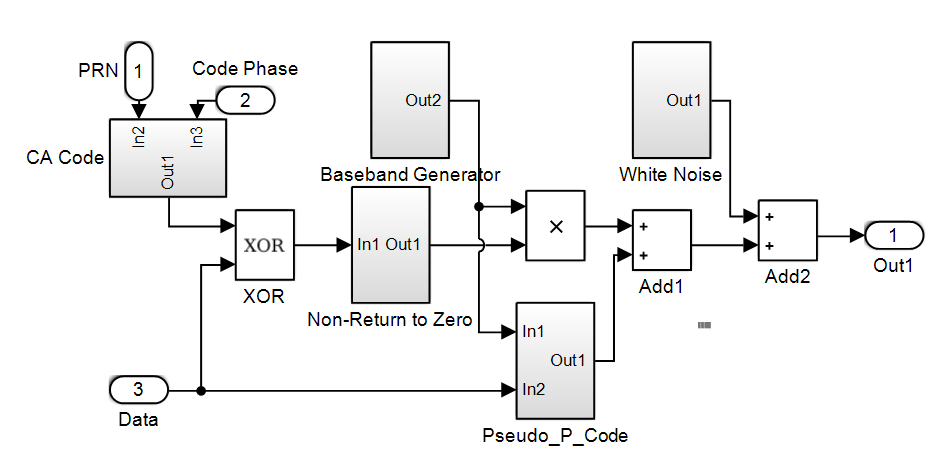
\includegraphics[width=\textwidth]{Signal_Generator}
		\caption{Signal Generator}
		\label{signal_generator}
	\end{figure}	
	
	The signal generator for testing tracking loops (Figure \ref{signal_generator}) is similar to the previous function generator used to test the acquisition loop\footnote{Detailed explanation of acquisition function generator available in previous semesters report}. Several additions and modifications made to the generator are explained below.
	
	\subsection{Simulated Doppler Shift}
	
	In order to properly simulate effects of the Doppler shift, a counter controlled VCO was used to generate the carrier signals. The counter begins at 0 and counts to 2500 over a one second period. Setting the VCO input sensitivity to $\pm$0.08,0.04, or 0.02Hz/V, allows us to achieve frequency shifts of $\pm$200, 100, or 50Hz/s respectively. A counter was also used to shift the C/A code phase by increments of $\frac{1}{32}$ (made possible by up-sampling and shifting the original code). Adjusting the sampling period of the counter, the desired code phase shifts of $\pm$3 to 6 chips/s can be produced.
	
	\subsection{Pseudo P-Code and Noise}
	
	A pseudo P-code was generated using a square wave with the same frequency of the actual P-code. This code is then modulated on to a 90 degree phase shifted carrier and tuned 3db down to better approximate actual GPS signal generation.
	
	The final addition to the signal generator was that of a white noise block. This allows  us to simulate noise that may occur in actual signals. We chose white noise specifically as it has equal intensity at different frequencies, providing a fairly uniform PSD. The ratio of signal to noise if varied between 10dB and 20dB 
	
	\section{Received Signal Demodulation}
	
	Once a signal has been determined to be in range by the acquisition stage, the data must be demodulated. To perform demodulation, it is required to multiply the incoming signal with a carrier-frequency matched local oscillator. This effectively wipes the carrier from the signal, bringing it back to the data baseband. The last step is to multiply the signal with a locally generated C/A code, effectively decoding the data.
	
	The values found during acquisition are used to generate the local oscillator and C/A code, however this is not enough. As explained above, the code phase and carrier frequency undergo Doppler shifts and change over time. These changes must be tracked and fed back to the generators to provide stable, coherent demodulation. The process of signal tracking is explained in the following section.
	\section{Tracking Loops}
	
	\subsection{Introduction}
	MOTIVATION\\	
	
	gps sig is bi-phase modulated\\
	
	carrier n code freqs change due to doppler effect from motion of gps satellite n receiver\\
	
	therfore to track gps signal requires 2 loops to be coupled together\\
	
	present/prompt code  code is applied to the digitized input
	signal and strips the C/A code from the input signal (by mult c/a code with signal at correct phase)
	
	output then is continuous wave with phase changes only from navigation data
	
	signal then applied to input of carrier loop and output is cw at carrier freq of input signal which is used to  strip the carrier from the digitized input signal,
	(mult this signal w  input signal)
	
	that output yields an output signal which is only a c/a code and no carrier freq which is then applied as the input to the code loop 
	
	
	.
	
	
	\subsection{Carrier Tracking}
	
	In order to successfully extract navigation data, a perfect replica of the carrier of the incoming signal must be used to demodulate the incoming signal and strip the carrier.
	A Phase Locked Loop (PLL) with a Voltage Controlled Oscillator (VCO) is used in GPS receivers to track the incoming signal's carrier and replicate it's frequency. The PLL employs a loop discriminator which produces a function of the error in the phase between the received signal and the local carrier. \\
	
	Since GPS signals are modulated using BPSK, a problem arises when using standard PLLs which are very receptive to the $180\degree$ phase shifts caused by the navigation data bit transitions.
	To ensure that our carrier tracking loop is insensitive to the phase transitions, we used a variation of the standard PLL called a Costas loop.
	
	\subsubsection{Costas Loop}
	
	The main feature of a Costas loop is its insensitivity to $180\degree$ shifts in phase [ref]. The input signal is multiplied with both the local carrier and a $90\degree$ phase shifted version of the carrier as shown in Fig \ref{Costas Carrier Tracking Loop}. The objective of the loop is to use the carrier loop discriminator and feedback in to the VCO  to keep all the energy in in the I (in-phase) arm.[REF] [Rewording needed]
	
	
	
	\begin{figure}[H]
		\centering
		\includegraphics[width=\textwidth]{Carrier_Tracking_Costas.png}
		\caption{Costas Carrier Tracking Loop}
		\label{Costas Carrier Tracking Loop}
	\end{figure}
	
	
	\subsubsection{Discriminators}
	
	A costas discriminator is used [to keep the energy in in phase arm] 
	
	
	\subsection{Code Phase Tracking}
	
	\subsubsection{Delay Locked Loop}
	
	\subsection{Discriminators}
	
	\subsection{Combined Tracking Loop}
	
	
	HELLO\\
	\begin{figure}
		\centering
		\includegraphics[width=\textwidth]{tracking_mdl.png}
		\caption{Combined tracking loop system block model}
		\label{Combined tracking loop system block model}
	\end{figure}
	
	
	
	
	
	\section{Simulink Implementation of Tracking Loop}
	
	\subsection{Simulink Model}
	
	The tracking loops implemented in simulink (Figure \ref{tracking_loop}) are modeled after a combined costas loop and delay locked loop mentioned in the previous section. The tracking stage block contains 4 of these loops, which track signal simultaneously 
	\begin{figure}
		\centering
		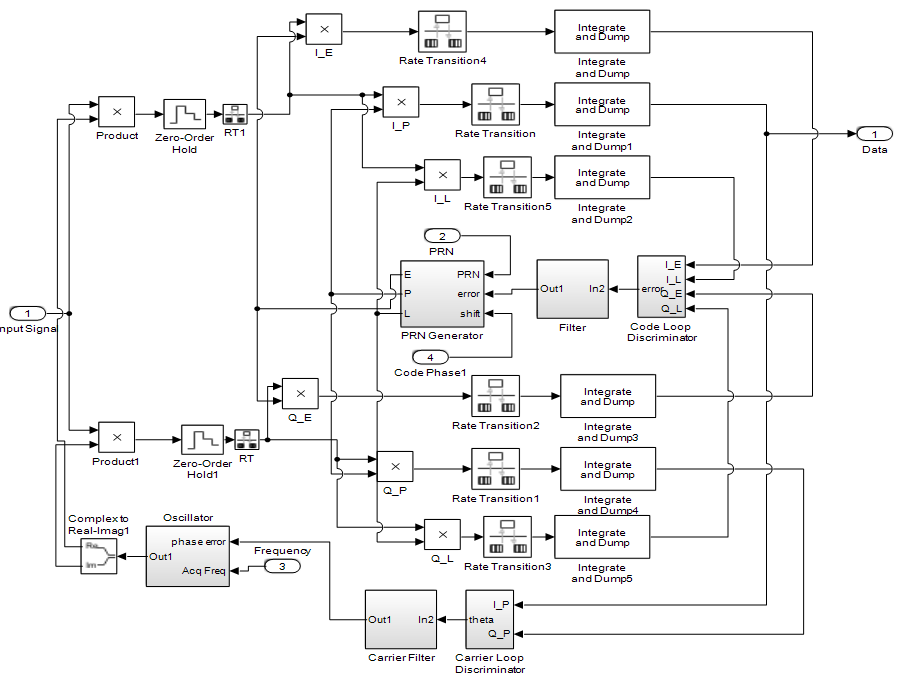
\includegraphics[width=\textwidth]{Tracking_Loop}
		\caption{Combined tracking loop simulink implementation}
		\label{tracking_loop}
	\end{figure}
	
	\subsection{Design Parameters}
	
	
	When transitioning from the block model to the simulink model, there are several design choices to be made. The error term used to drive the local oscillator for carrier tracking is an arctan discriminator. This provides indifference to the $180\deg$ phase shifts seen in BPSK signals. The error term used to drive the C/A code generator is the normalized early minus late power discriminator. This discriminator provides the best tracking when chip errors are larger than one. The integration period of the integrate and dump block is 1ms, equal to one full C/A code. In order the perform the necessary signal processing in discrete time, the continuous input signal was converted using a zero order hold block with a sampling rate equal to the sampling rate of our system ($f_{s}$=32.768MHz).
	\subsection{Controlled Oscillator}
	The controlled oscillator used to wipe the carrier from the signal is modeled after a numerically controlled oscillator. The NCO takes as input a phase error term which provides a phase increment. This increment is added to an internal phase accumulator whose value is used to output a sine wave of the correct frequency. The formulas used to control the output of the NCO are provided below. Note that the accumulator word length (N) is 16 for our implementation.
	
	The frequency of the output is $f_{0}=\frac{\Delta\theta f_{s}}{2\pi 2^{N}}$, 	
	where $\Delta\theta[n]=2\pi 2^{N}(\frac{f_{c}}{f_{s}}+e[n])$
	
	The output of an NCO can be written as \begin{equation}\cos[n] = \cos(2\pi[n\frac{f_{c}}{f_{s}}+\sum\limits_{i=0}^n e[i] ])
	\end{equation}
	Using this relationship between error term and NCO output, A simulink model for the local oscillator was created as shown in Figure \ref{NCO}.
	\begin{figure}
		\centering
		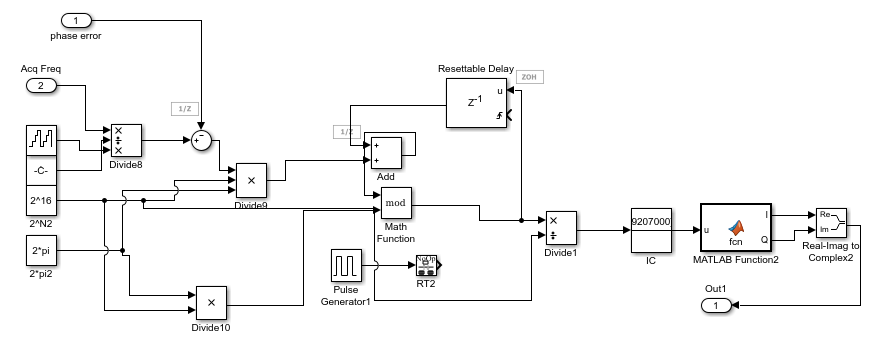
\includegraphics[width=\textwidth]{NCO}
		
		\caption{Tracking Loop Locally Generated Oscillator}
		\label{NCO}
	\end{figure}
	
	\subsection{Controlled C/A Code Generator}
	\begin{figure}
		\centering
		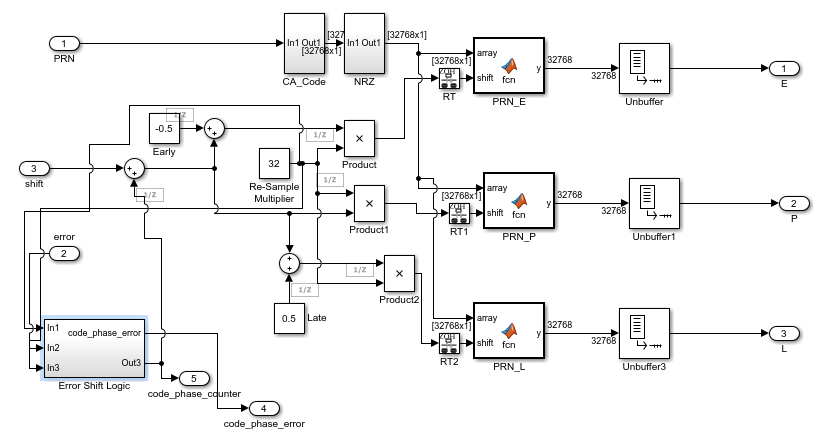
\includegraphics[width=\textwidth]{Tracking_CA_Code}
		
		\caption{Tracking Loop C/A Code Generator}
		\label{TCA}
	\end{figure}
	The C/A code generator (Figure \ref{TCA}) is modeled after that of the acquisition stage, with a few adjustments. To make use of our desired discriminator, we must produce an early and late version of the C/A code ( spaced half a chip apart) in addition to the prompt code. To space the chips properly, the C/A code is up sampled 32 times and shifted 16 bits away from the correct code phase, in the appropriate direction. The error term of the code phase discriminator is then added to the detected code phase from acquisition, allowing tracking of the correct code phase to be input to the local C/A code generator.
	
	\subsection{Discriminator Filtering}
	
	In order to provide smooth changes to the local carrier generator, the error term must be filtered. The filter implemented in simulink consist of a simple second order IIR filter. The fixed parameters used to choose appropriate coefficients are
	
	\begin{description}
		\item[Bandwidth] 30Hz	
		\item[Damping Coefficient] 0.707
		\item[Loop Gain] $\frac{1}{4}$		
	\end{description}
	
	The set values of these parameters were chosen based on resulting waveforms of the carrier discriminator for several test values. 
	The actual coefficients used in the IIR fiter block can then be calculated by using the following formulas:
	$ formula $
	
	
	\section{Tracking Loop Testing}
	
	To test the full functionality of the tracking stage, we must first test each individual parameter. Certain parameters were tested as the loop was being built, however that is not enough to guarantee proper functionality. To thoroughly validate requires us to generate a few test signals to work with. A real GPS signal would use data bits of 50Hz, however, for the purpose of saving time on simulations we have set it to 100Hz. Data bit values are set according to a 5 bit repeating vector unique to each generated signal. The defining features of our test signals are listed below, where the value in brackets indicates the doppler shift.
	
	
	\begin{table}
		\begin{center}
			\begin{tabular}{||c c c c||}
				\hline
				Satellite Number & Carrier Frequency & Code Phase &Data Vector	\\
				\hline\hline
				1 & 9.209MHz (+50Hz/s) & 0 (+3chips/s) & [1 0 0 1 1] \\
				\hline
				2 & 9.204Hz (-100Hz/s) & 200 (+3chips/s) & [1 0 1 0 1]\\
				\hline
				3 & 9.207MHz (+200Hz/s) & 512 (-3chips/s) & [0 1 1 0 0]\\
				\hline
				4 & 9.207MHz (+100Hz/s) & 999 (+3chips/s) & [1 0 0 1 0]\\
				\hline
			\end{tabular}
			\caption{Test Signal Parameters}
			\label{tsp}
		\end{center}
	\end{table}
	
	Normally the satellite PRN number, code phase and carrier frequency would be passed to the tracking loop from the acquisition stage, however for the purposes of testing, these parameters are pre-set and loaded in from a matlab array.
	
	The very first test involving the tracking stage was simply to demodulate the data from a single signal when no other signals are present. This is fairly straightforward as the tracking loop should be able to demodulate data in the beginning without worrying about tracking changes. This beginning test was successful in recovering the generated data, and we were able to move on to the next stage of testing. 
	In the following sections when discussing tracking results, signals are referred to by the order they appear in their respective legends.
	
	\subsection{Carrier Tracking Testing}
	
	The first carrier tracking test involved a single test signal, feeding the tracking loop with the exact values used to generate it. As the signal propagates, the frequency will changing, and we must look at a plot of the discriminator error term to determine whether it is being tracked accurately. The resulting shows two tracking loops, one where error feedback is implemented, and the other where it is now.
	
	\begin{figure}
		\centering
		\label{Carrier_Tracking_Test_1}
		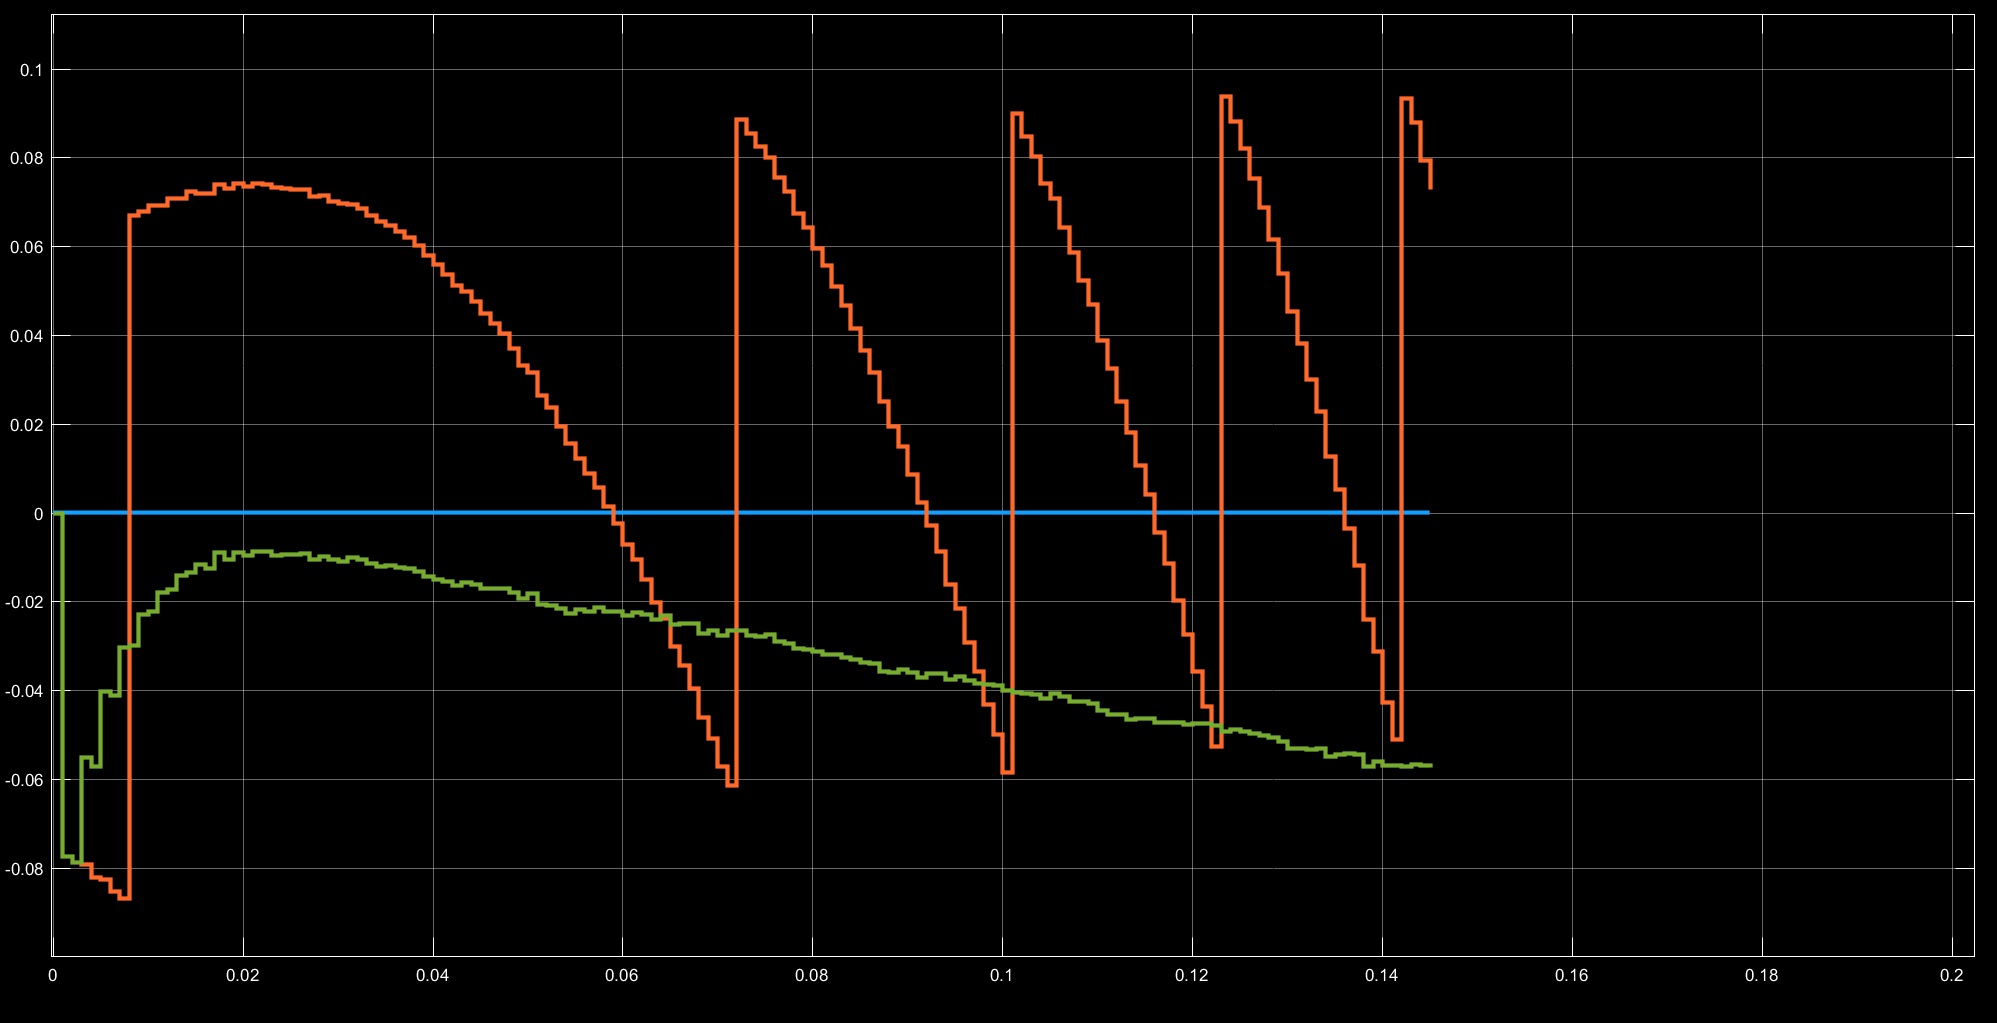
\includegraphics[width=\textwidth]{Carrier_Tracking_Test_1}
		\caption{Carrier tracking error term for single signal test}
		\label{carrt1}
	\end{figure}
	
	As can be seen in Figure \ref{carrt1}, when the error term is fed back into the carrier generator, the loop is able to accurately track its changes. When feedback is not enabled however, the loop quickly looses track of the signal.
	
	The second carrier tracking test involved feeding four different tracking loop with the same signal, but deviating the supplied initial carrier frequency. These deviations were 1000Hz, 500Hz, and 250Hz shifts from the actual carrier frequency of 9.207MHz.
	
	\begin{figure}
		\centering
		\label{Carrier_Tracking_Test_2}
		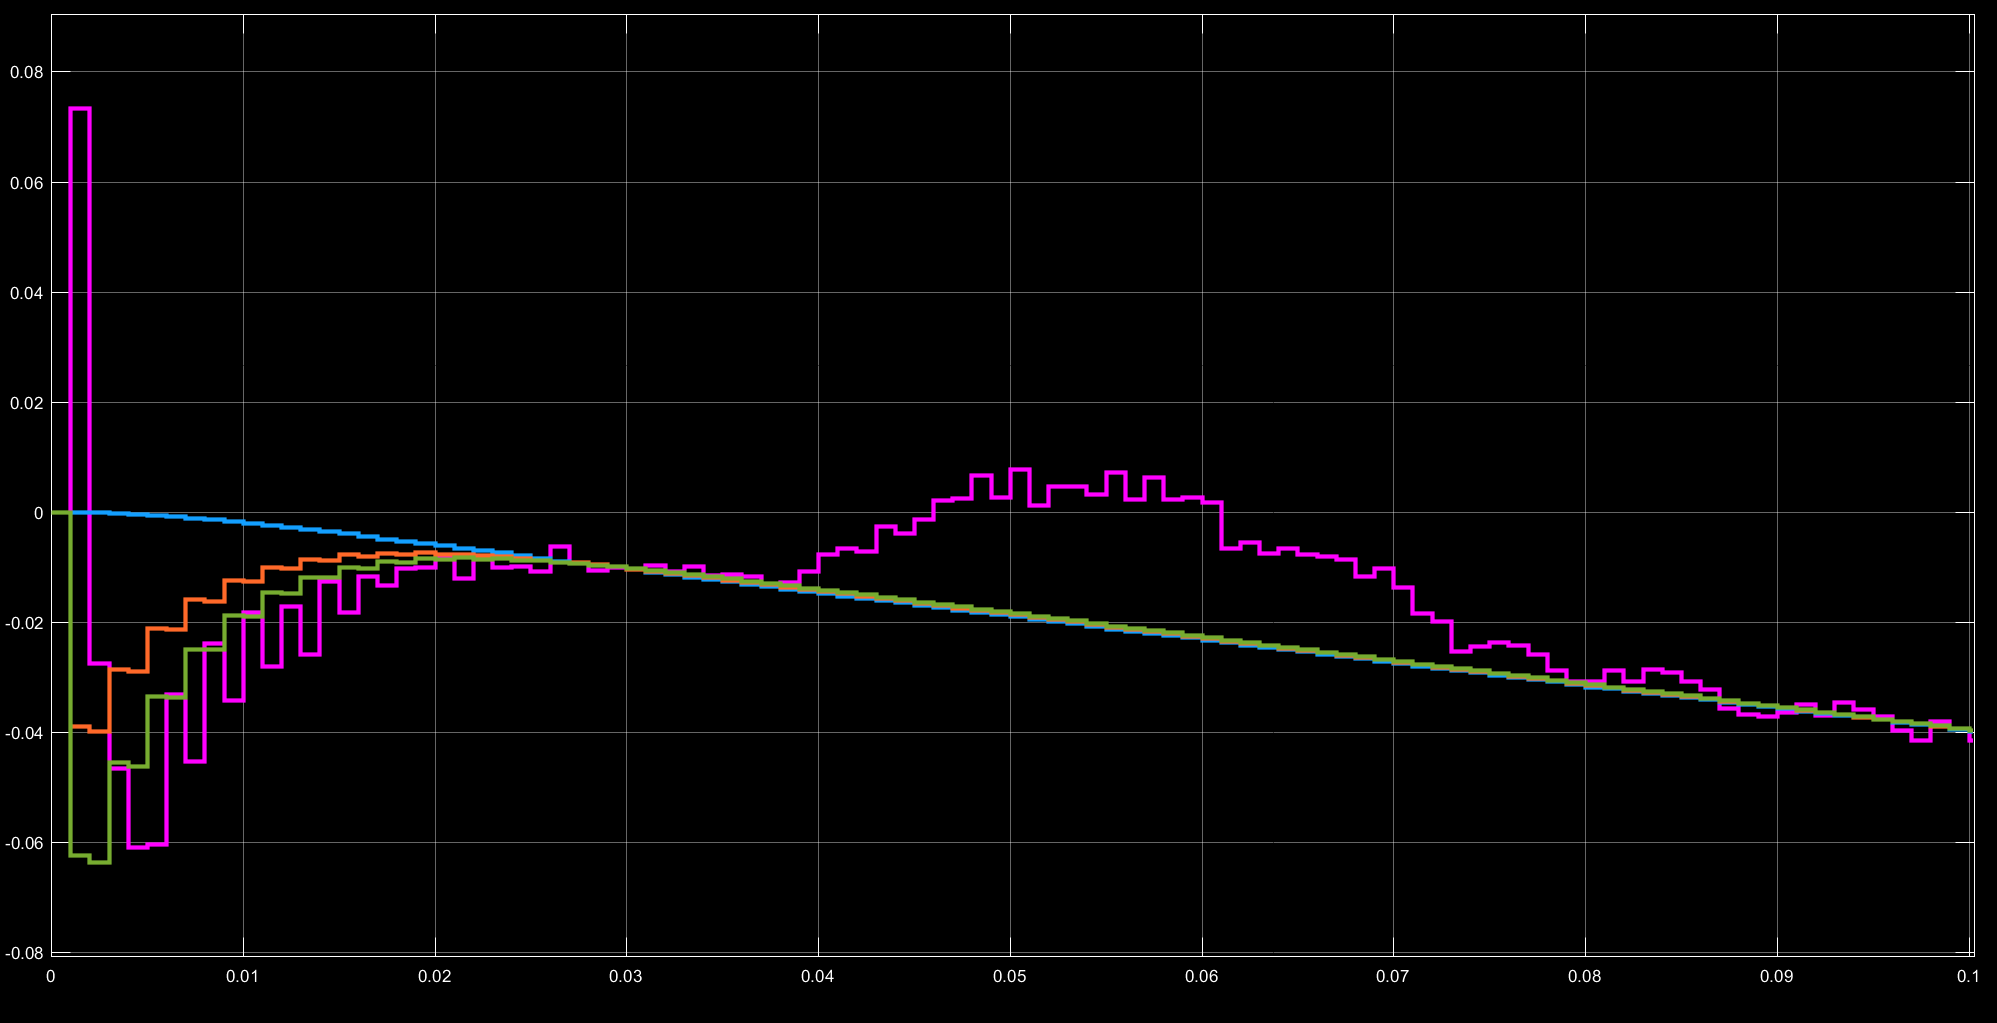
\includegraphics[width=\textwidth]{Carrier_Tracking_Test_2}
		\caption{Carrier tracking error term for single signal with varying initial frequencies}
		\label{carrt2}
	\end{figure}
	
	As can be seen in Figure \ref{carrt2}, the carrier loops are able to track on to the first 3 signals is under 30ms. The farther off the supplied frequency is from the actual value, the longer it takes to settle. However, for the loop being fed with a frequency off by 1000Hz, the lock in is never achieved. 
	
	The final carrier tracking test was carried out using an input signal consisting of a sum of all 4 generated signals. The purpose of this testing stage is to determine whether or not the loop can properly track the changes to four different signal being received at the same time. Achieving this will help to ensure that the system will coherently demodulate data from multiple signals in final testing.
	
	The test signals used to generate \ref{carrt3} are the ones listed at the beginning of this section in \ref{tsp}, and correspond to the order they appear in the legend of the plot.
	
	\begin{description}
		\item[Signal 1]{ +50Hz/s}
		
		\item[Signal 2]{ -100Hz/s}
		
		\item[Signal 3]{+200Hz/s}
		
		\item[Signal 4]{100Hz/s}
	\end{description}
	
	\begin{figure}
		\centering
		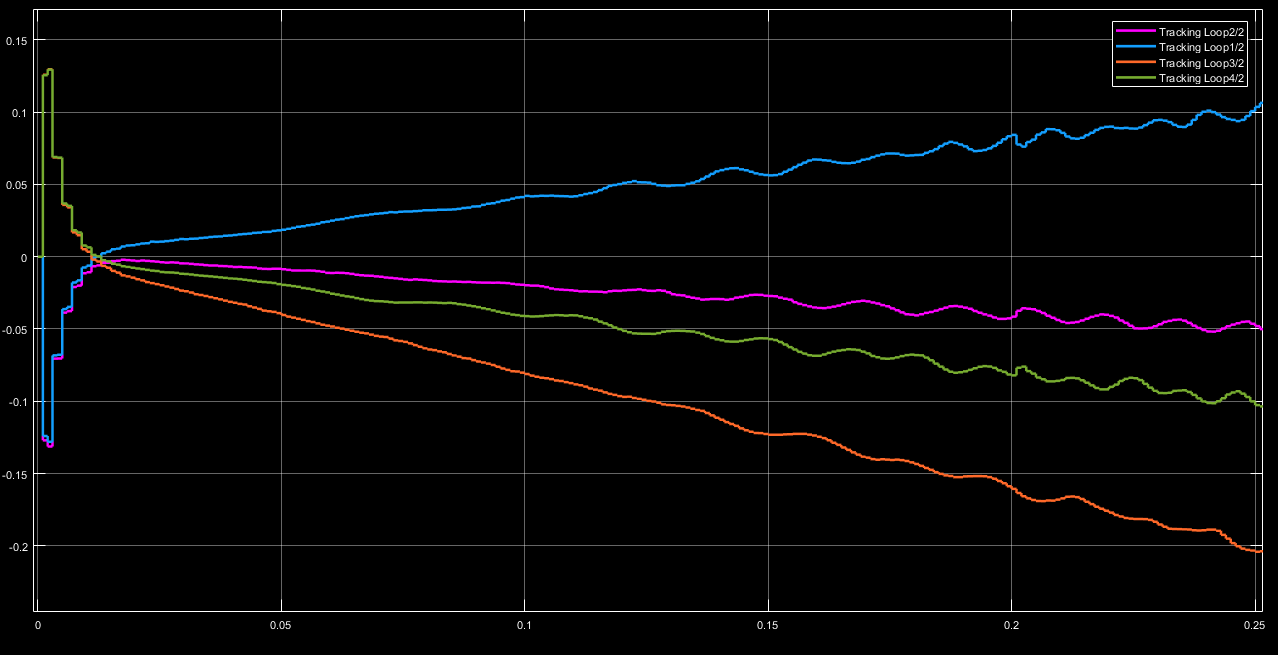
\includegraphics[width=\textwidth]{Carrier_Tracking_Test_3}
		\caption{Carrier tracking error term for 4 different signals}
		\label{carrt3}
	\end{figure}
	
	To validate the function of this loop, we must observe the slope of the signals plotted in Figure\ref{carrt3}. Since the slopes of each signal match approximately to their doppler rate, It is evident that the tracking system is able to accurately measure changes to one signal in the presence of others. We must now test the remaining tracking loop functions.
	\subsection{Code Phase Tracking Testing}
	
	Code phase tracking was carried out in a manner similar to carrier tracking. The initial code tracking test involved a single signal, feeding the tracking loop with the exact code phase value used to generate the test signal. As the time passes, the code phase will changing, and we must look at a plot of the code discriminator error term to determine whether it is being tracked accurately. The plot below shows two code tracking loops, one where error feedback is implemented, and the other where it is not. 
	
	\begin{figure}
		\centering
		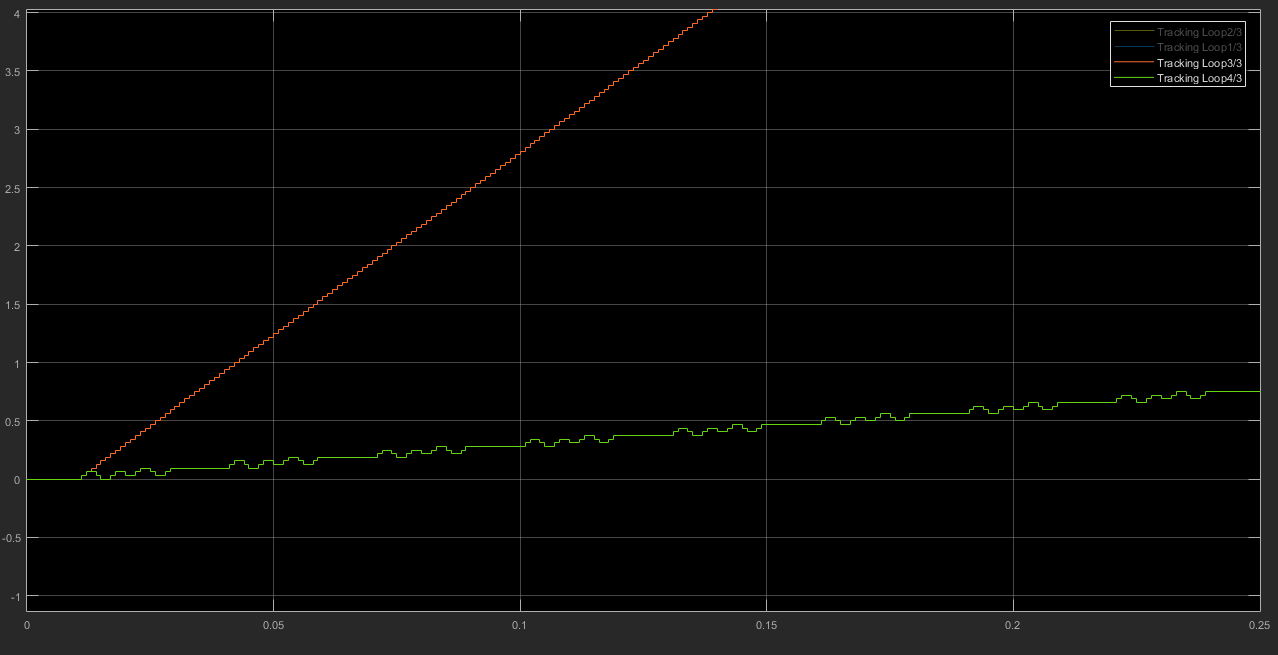
\includegraphics[width=\textwidth]{Code_Tracking_Test_1}
		\caption{Code tracking error term for single signal}
		\label{code1}
	\end{figure}
	
	As observed in Figure \ref{code1}, when the error term is fed back into the carrier generator, the loop is able to accurately track its changes. When feedback is not enabled however, the loop quickly looses track of the signal.
	
	
	The second carrier tracking test involved feeding four different tracking loop with the same signal, but deviating the supplied initial carrier frequency. These deviations were 0 chips, 1 chip, 3 chips and 5 chips away from the actual code phase of 1000.
	
	\begin{figure}
		\centering
		\label{Code_Tracking_Test_2}
		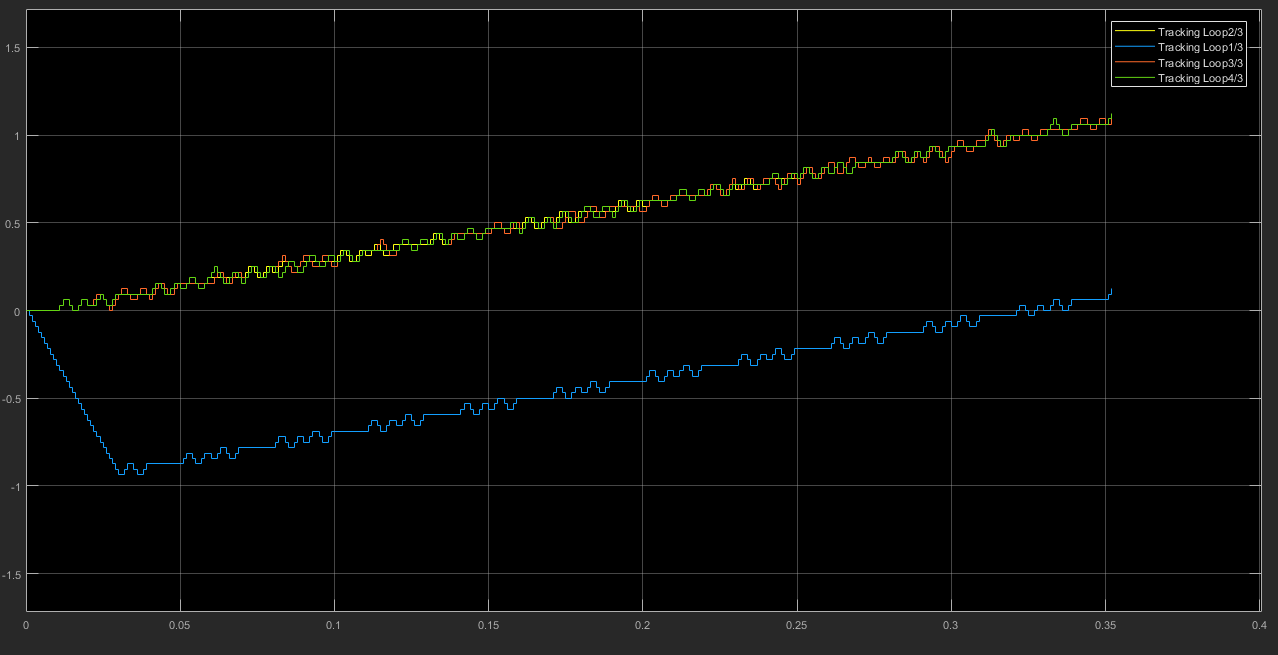
\includegraphics[width=\textwidth]{Code_Tracking_Test_2}
		\caption{Code tracking error term for single signal with varying initial code phases}
		\label{code2}
	\end{figure}
	\FloatBarrier
	As can be seen in Figure \ref{code2}, the code loops are able to track on to signal with a one chip shift in approximately 30ms. For code phase errors of more than two chips, the loop failed to lock in. This may perhaps be improved upon with a different method of adjusting the C/A code, or better smoothing of the error term. In all test cases however the C/A code phase was always correct so we should not have to worry about the code phase suddenly shifting more than two chips.  
	
	
	The final code tracking test was carried out using an input signal consisting of a sum of all 4 generated signals. The purpose of this testing stage is to determine if the loop can track changes to four different signals being received at the same time. Achieving this will help to ensure that the system will coherently demodulate data from multiple signals in final testing.
	
	The test signals used to generate Figure \ref{code3} are the ones listed at the beginning of this section in Table \ref{tsp}, and correspond to the order they appear in the legend of the plot.
	
	\begin{description}
		\item[Signal 1]{ +3chips/s}
		
		\item[Signal 2]{ +3chips/s}
		
		\item[Signal 3]{-3chips/s}
		
		\item[Signal 4]{+3chips/s}
	\end{description}
	
	\begin{figure}
		\centering
		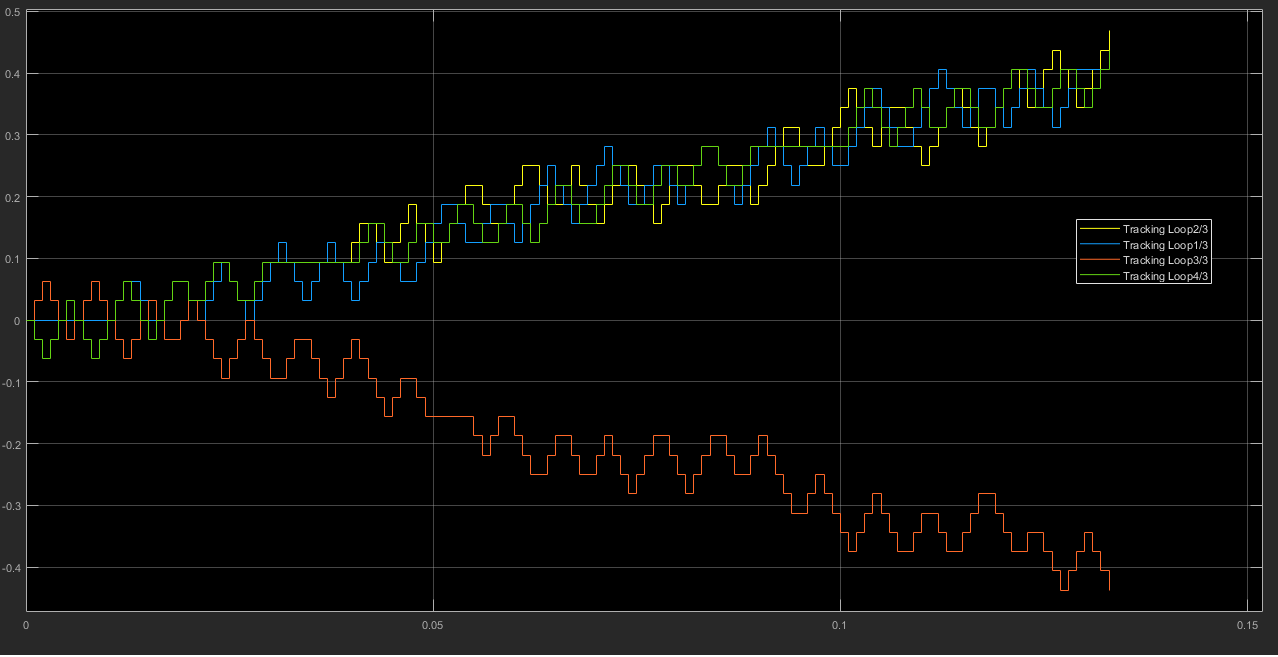
\includegraphics[width=\textwidth]{Code_Tracking_Test_3}
		\caption{Code tracking error term for single signal with varying initial code phases}
		\label{code3}
	\end{figure}
	\FloatBarrier
	To validate the function of this loop, we must observe the code phase error signals plotted in Figure\ref{code3}. Since the slope of the average of each signal has an approximate linear relation to the doppler shift rate, it is evident that the tracking system is able to accurately measure changes to one signal in the presence of others. We must now test the carrier and code tracking loops together.
	
	\subsection{Combined Signal Testing}
	The last test needed to complete the validation of our tracking stage involves summing 4 different signals as input. The signal parameters are passed to tracking from a pre-set array with initial values; These values represent the test signal parameters (as seen in Table \ref{tsp} . The goal of this final stage is to recover the transmitted data bit vectors listed below.Note that the signals are numbered by their order of appearance in the plot legend. 
	\begin{description}
		\item[Signal 1]{[1 0 0 1 1]}
		
		\item[Signal 2]{[[1 0 1 0 1]]}
		
		\item[Signal 3]{[0 1 1 0 0]}
		
		\item[Signal 4]{[1 0 0 1 0]}
	\end{description}
	
	
	\begin{figure}
		\centering
		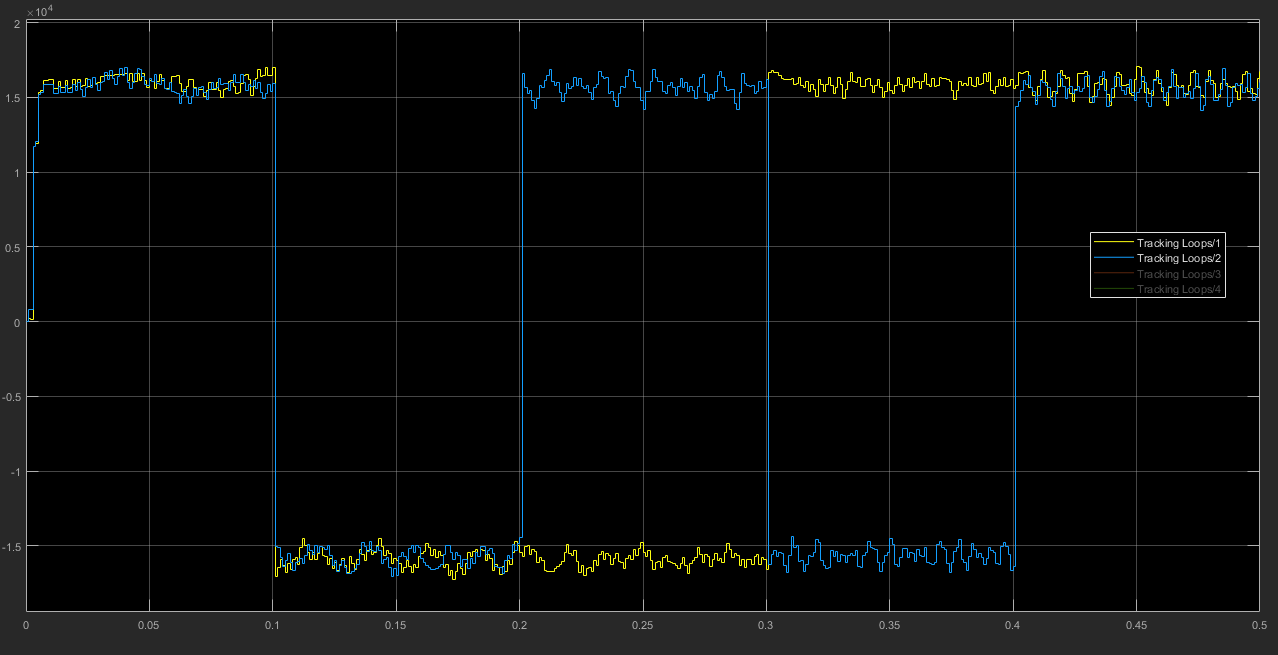
\includegraphics[width=\textwidth]{Tracking_Test_Full_1}
		\caption{Final Tracking Loop Test Result Plot}
		
		\label{dmod1}
	\end{figure}	
	
	\begin{figure}
		\centering
		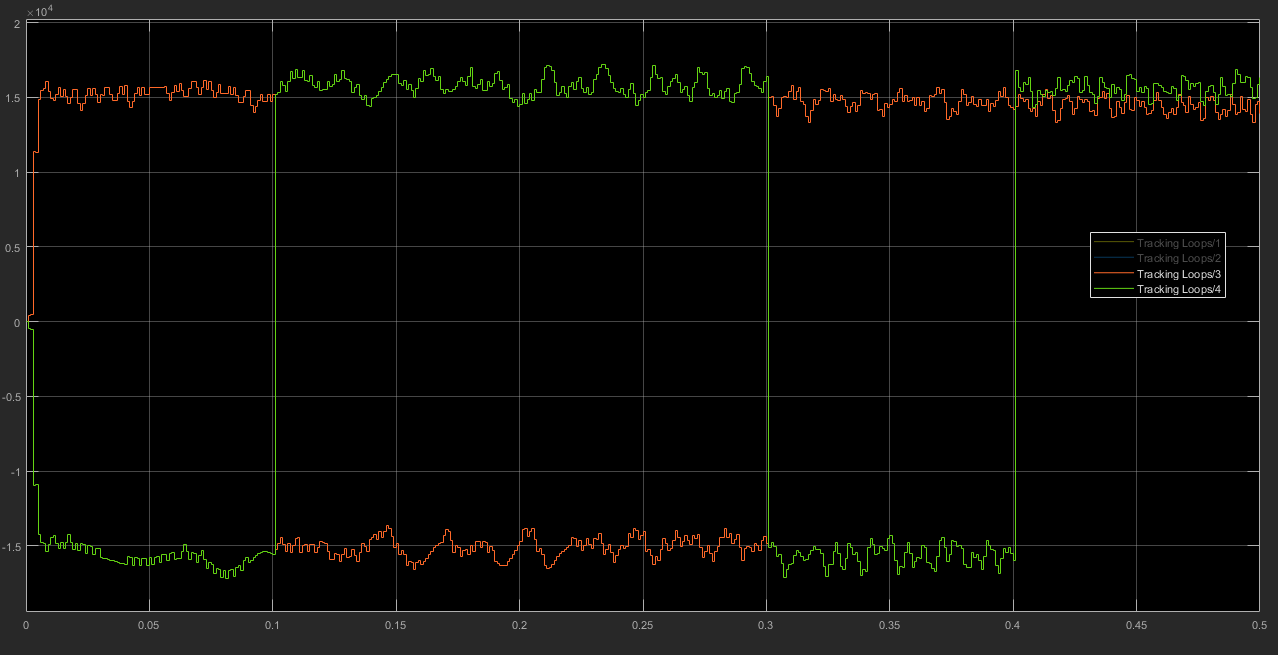
\includegraphics[width=\textwidth]{Tracking_Test_Full_2}
		\caption{Final Tracking Loop Test Result Plot}
		
		\label{dmod2}
	\end{figure}	
	
	Figure \ref{dmod1} shows the resulting demodulate waveform for signals 1 and 2, while Figure \ref{dmod2} shows the resulting waveform for signals 3 and 4. The signals only exhibit sign (bit) changes every 0.1s (100Hz) which is the rate of data that we chose when generating the signal. This is the first sign that demodulation is being performed properly. Another good sign is the lack of correlation attenuation over time. If the loop were not performing properly this correlation value would drop over time towards zero. The last step of validation is to match the generated data vectors to their demodulated signals. Note that the demodulated waveform is in the non-return to zero format (on the set [-1,1]). Through visual comparison it is clear that the vectors do all indeed match up correctly, however the bits have been inverted for signals 3 and 4. This is perfectly fine however, as it is a property of working with BPSK signals which are encoded with a $180\deg$ phase shift. The bit inversion must be detected by the data navigation extraction stage before any useful data can be extracted. 
	\section{Synthesis with Acquisition Stage}
	
	\begin{figure}
		\centering
		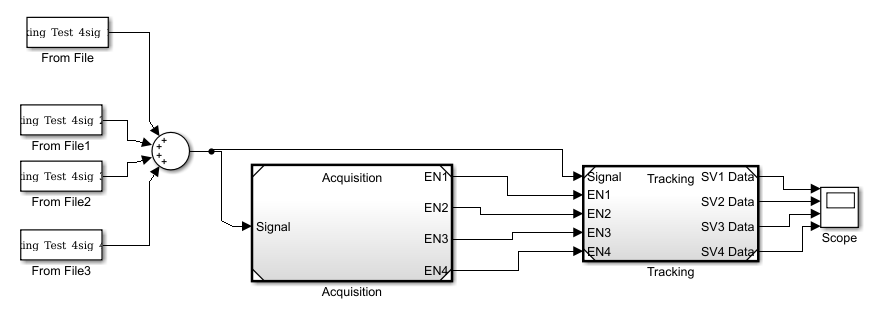
\includegraphics[width=\textwidth]{Receiver_Model}
		\caption{Synthesized receiver model}
		\label{FRec}
	\end{figure}	
	
	The final phase of this project was to test both the acquisition and the tracking stages together. The information used for tracking initializations must now come from the acquisition results instead of being pre-set (as in previous testing stages). To make this synthesis function as intended, some overhead logic is needed to control both models, as well as store and sort satellite parameters. Testing results and details of the adjustments required to successfully synthesize both models is provided in the following sections.
	\subsection{Adjustments to Acquisition and Tracking}
	
	\begin{figure}[h]
		\centering
		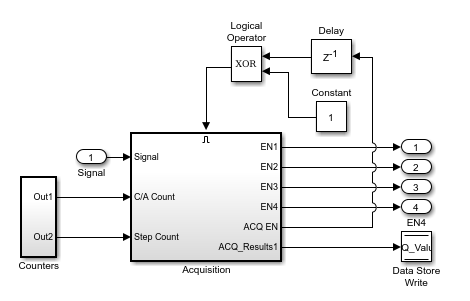
\includegraphics{Acquisition_Logic}
		\caption{Overhead logic used to control acquisition model}
	\end{figure}	
	
	
	To gather useful information from the correlation output, a matlab function block was written which stores the code phase of the highest correlation value at every frequency step. The largest value per C/A code is found in a similar manner, allowing us to locate both the code phase and frequency step of the highest correlation peak. If this peak is determined to be above our threshold ($2*10^{7}$, found through correlation data analysis) it is added to an array of acquired signals.
	
	As the array is filled, the signals should be organized according to signal strength; This can be achieved by looking at either correlation peaks or the SNR value. The organized array is then output from the loop, where it is written to a variable via a data set memory block. This shared memory block will then be read out during tracking and used to initialize the loop parameters, as shown below.
	\begin{figure}[!h]
		\centering
		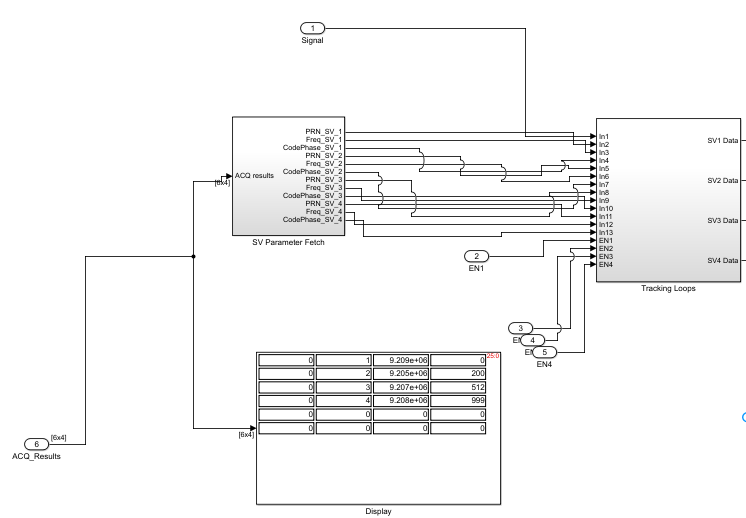
\includegraphics[width=\textwidth]{Tracking_Loop_2}	
		\caption{Tracking loop initialization}
	\end{figure}	 
	
	The acquisition block controls the start of tracking stage execution through a wired boolean enable line. The acquisition loop will also terminate itself when it is no longer needed. The tracking stage of a real GPS receiver would ordinarily not start until the best suited satellites are found, which requires a full sweep through the 24 possible satellites orbiting the earth. For the purposes of our testing however, the acquisition stage will enable the tracking of signals as they are found. This allows us to reduce the computation time required to view the results of tracking.
	\subsection{Final Test}
	The final test was performed on the sum of 4 generated signals. Unlike previous tests, this time all of the tracking initialization parameter values come from the results of the acquisition stage. All of the signals have a data rate of 100Hz (real GPS uses 50Hz, changed to reduce required computation time) as well as different 5 bit repeating data vectors. The goal of this final stage testing is to simply provide an input signal and see if the recovered data bits match the generated ones. 
	
	\begin{figure}
		\centering
		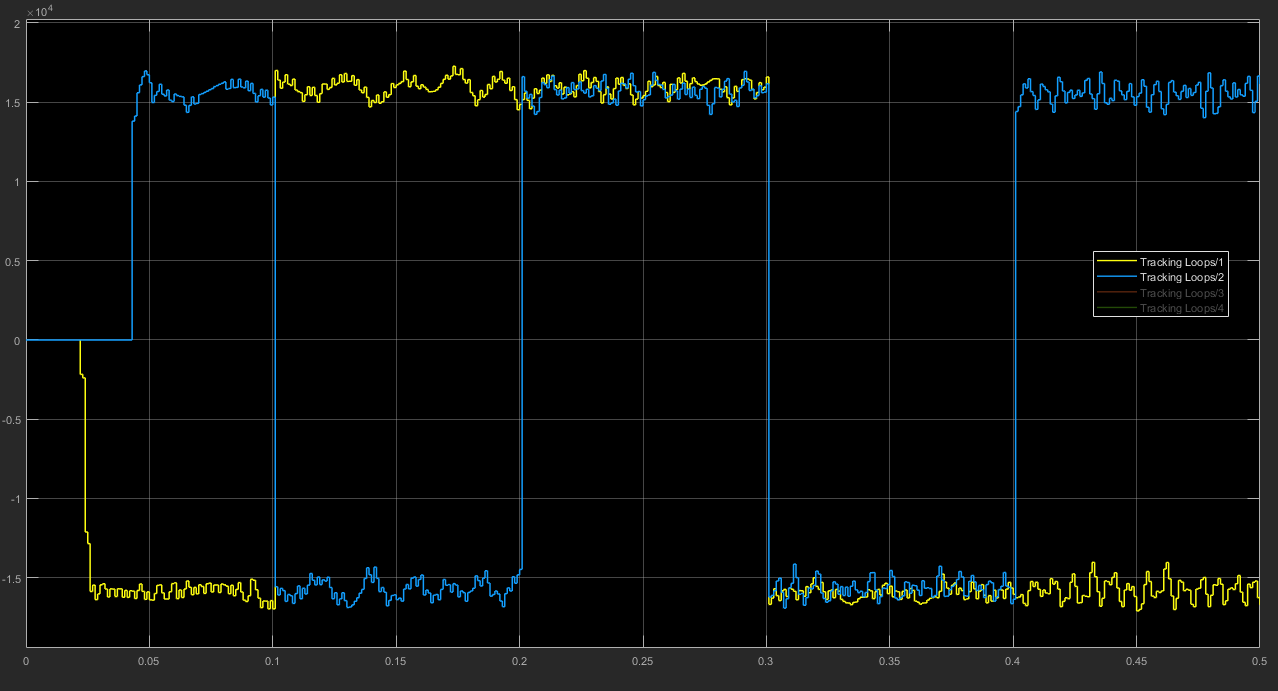
\includegraphics[width=\textwidth]{Synth_Test_Data_1}
		\caption{Receiver Model Data Results Signal 1 \& 2}
		\label{RD1}
	\end{figure}	
	
	\begin{figure}
		\centering
		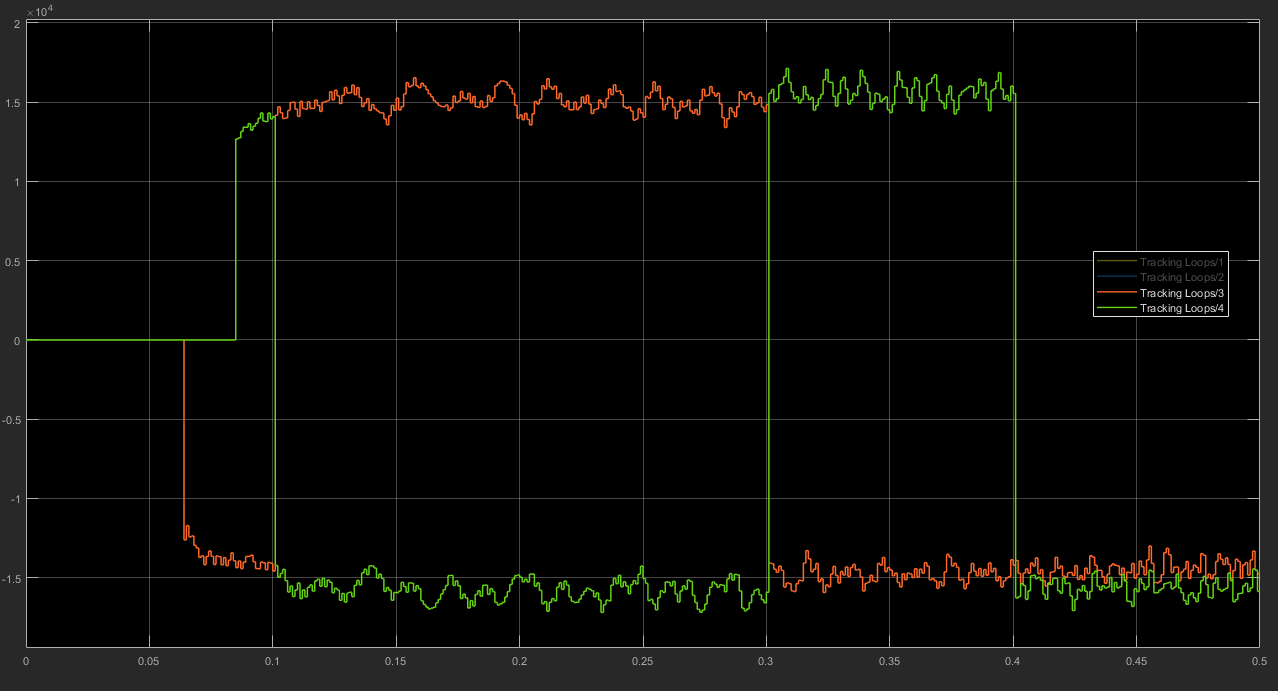
\includegraphics[width=\textwidth]{Synth_Test_Data_2}
		\caption{Receiver Model Data Results Signals 3 \& 4}
		\label{RD2}
	\end{figure}	
	\FloatBarrier
	\begin{figure}
		\centering
		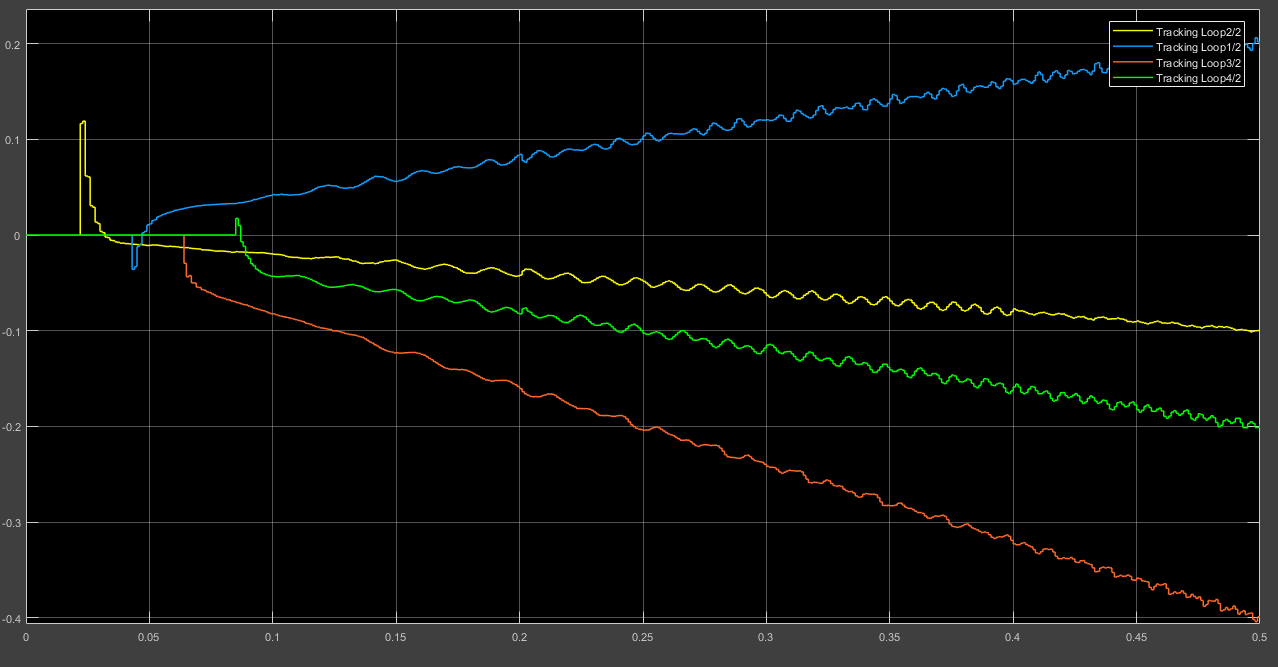
\includegraphics[width=\textwidth]{Synth_Test_Carr}
		\caption{Receiver Model Carrier Discriminator Output}
		\label{RCarr}
	\end{figure}	
	
	\begin{figure}
		\centering
		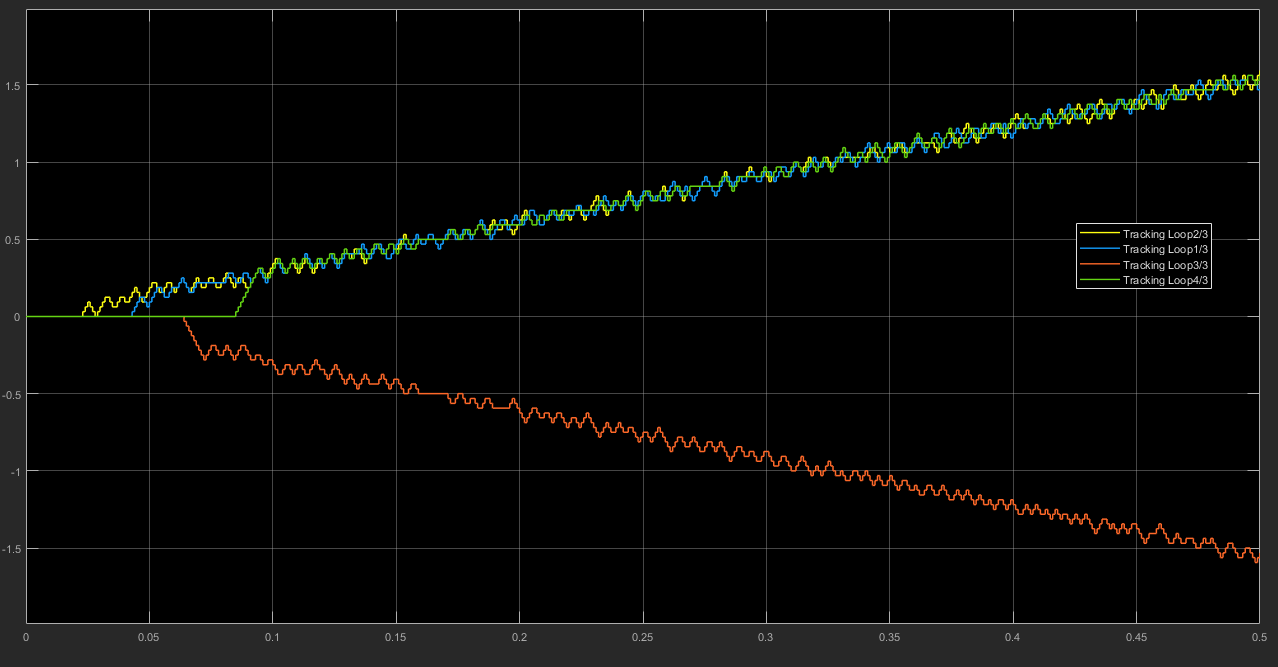
\includegraphics[width=\textwidth]{Synth_Test_Code}
		\caption{Receiver Model Code Discriminator Output}
		\label{RCode}
	\end{figure}	
	
	
	The resulting plots of carrier discriminator (Figure \ref{RCarr}), code discriminator (Figure \ref{RCode}) and demodulated data bits (Figures \ref{RD1} \& \ref{RD2}) show a delay in signal tracking from simulation start time. This delay is caused by the time taken for acquisition to find each signal and pass on the parameters, enabling the tracking loop to begin. The demodulated data, carrier discriminator and code discriminator values agree with the previous values of tracking stage testing, as well as the generated values. Through this final simulation we have validated that our system does indeed work as designed.  
	
	\section{Data Navigation Extraction Overview}
	The output of the tracking stage is the in-phase arm of of the tracking block. These values need to be truncated to the set of [-1,1] (based on their sign). Due to noise or weak signals the values will be slightly distorted, so the mean value over 20ms (data rate) should be used to truncate values.The next step is to determine when a bit transition happens by detecting a zero crossings. Once the beginning of a bit transition is known, the 1000Hz samples from tracking can be correctly down-sampled to 50Hz navigation data bits.
	
	After the data has been properly converted, the beginning of a subframe must be located. This is marked with an 8-bit preamble of [10001011]. As mentioned earlier the costas loop is invariant to $180\deg$ phase shifts, leading to possible bit inverted version of [01110100]. Correlating the incoming data with this preamble will determine when the data sub frame starts, and whether the bits are inverted or not.
	
	Each sub frame contains 300 bits divided into 10 words of 30-bits each. 24 bits of each word contain actual data, while the rest belong to a 6-bit parity. This parity is used to confirm whether data whether received data was interpreted correctly. If the parity check is successful the navigation data can be decoded using information provided in the ICD-GPS-200. The decoded data can then be used for the required calculations to determine position.
	
	\section{Impact on Society and the Environment}
	\section{Report on Teamwork}
	
	\section{Conclusion}
	
	\section{References}
	
	\section{Appendix}	
	
	
	
\end{document}
